\documentclass[10pt,a4paper,final]{scrartcl}
\usepackage[utf8]{inputenc}
\usepackage{amsmath}
\usepackage{amsfonts}
\usepackage{amssymb}
\usepackage{graphicx}
\usepackage{float}
\author{
Group No.: 05 \\ 
Group Members: \\
LIU Xinhong (53043714) \\
LI Tong (53043505) \\
ZHONG Yuqing (53057522)
}
\titlehead{
City University of Hong Kong \\
Department of Electronic Engineering
}
\title{
EE3316 Information Product Design \\ Mobile App Design Final Report \\ Into Heart}
\subtitle{2013/14 (Semester B)}
\begin{document}
\maketitle

\pagebreak

\begin{abstract}
Heart is a vital organ of human body, once it stops, no matter how strong, you are gone.  
This app monitors heart rate all-day and evaluate heart health condition, integrates into everyday exercise training session and help user to control the exercise strength, to reach a better exercise goal, as well as training heart. With social integration, this app connects user with friends and family to motivate user care about their heart. This app also conducts emergency alert including: contacting the family, call ambulance, make noise, or any other viable first aids. 
\end{abstract}



\tableofcontents

\section{Introduction}

\subsection{Market Research}

Cardiovascular diseases (CVDs) are a group of disorders of the heart and blood vessel. In 2012 it kills 17 million people, makes 31\% of all death in the world\footnote{WHO, Cardiovascular diseases (CVDs), retrieved from http://www.who.int/mediacentre/factsheets/fs317/en/ on Feb 2, 2015 }. 
According to some researches, heart rate (HR) is an independent predictor of cardiovascular and all-cause mortality in men and women with and without diagnosed cardiovascular disease1. Heart rate was assigned the same weighting as blood pressure and cardiorespiratory fitness in the overall score1. On the other hand, It's vital to monitor your heart rate during exercise3. A target heart rate is recommended to reach best exercise goal. Time is important when heart attack suddenly occur, time is life, handling emergency situation is a problem when patient is not near there relatives. 

\subsection{App Summary}
\subsection{Target User Group}
\subsection{Competitive Analysis}

\section{App Design and Analysis}
\subsection{Architectural Design}
\begin{figure}[H]
\centering
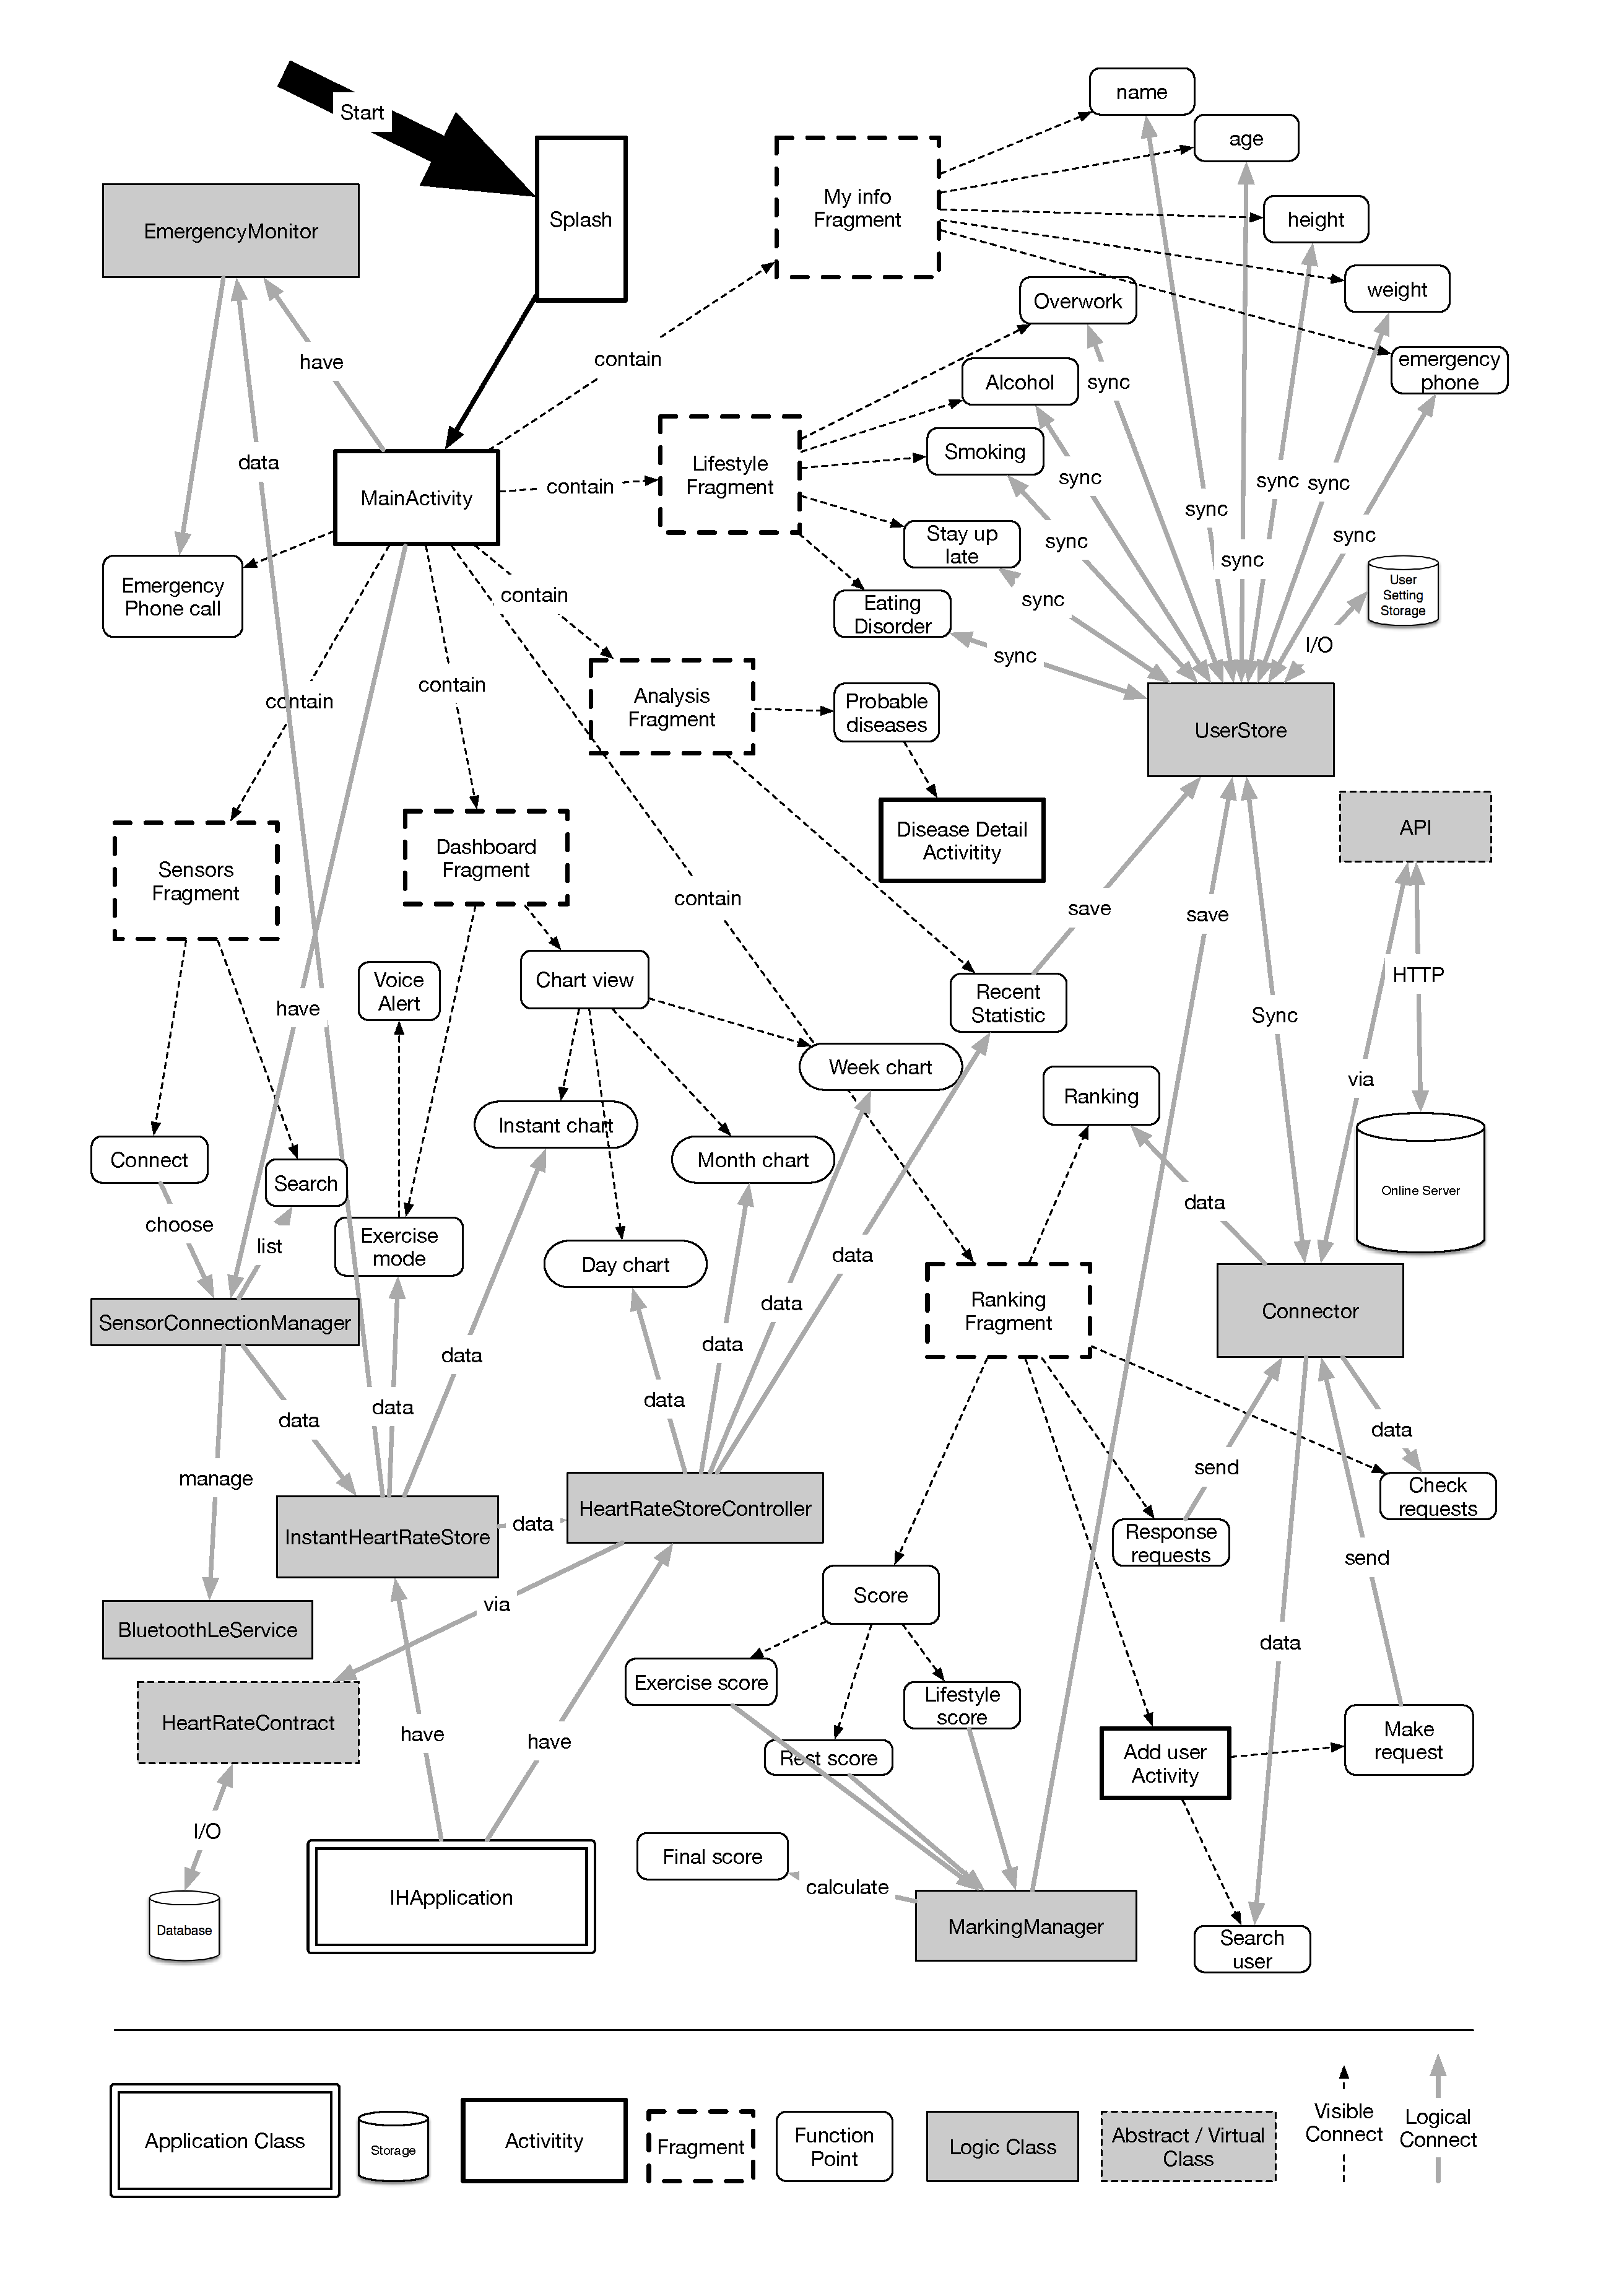
\includegraphics[width=5.3in]{img/arch.eps}
\caption{Into Heart Architectural Design}
\end{figure}

\section{Configuration}
\subsection{Configuration}
\subsubsection{App}
For Into Heart App, we use Android Studio project structure with Gradle project automation tool to do package management. The project bone structure is as followed.

\paragraph{IHApplication} is the Application class and holds global variables.
\paragraph{MainActivity} is the main activity with a navigation drawer to navigate between fragments, also the inner class EmergencyMonitor monitor heart rate and make emergency call when necessary.
\subparagraph{NavigationDrawerFragment} is navigation drawer fragment, let user navigate between fragments.
\subparagraph{DashboardFragment} is under MainActivity and let users view the instant heart rate and historical charts, as well as exercise mode.
\subparagraph{AnalysisFragment} is under MainActivity and let users view their recent heart rate analysis result  and the diseases they might have.
\subparagraph{SensorsFragment} is under MainActivity and let users search the sensors nearby and connect to them.
\subparagraph{RankingFragment} is under MainActivity and let user view their score and the ranking among friends. Searching friends, sending friend requests and responding the requests are in this fragment.
\subparagraph{UserInfoFragment} is under MainActivity and let user set their basic informations such as name, age, weight, height and emergency telephone.
\subparagraph{LifestyleFragment} is under MainActivity and let user rate their lifestyle, including smoking, alcohol, eating disorder, stay up late and overwork.
\paragraph{AddFriendActivity} can be entered from RankingFragment, letting user search and send friend request.
\paragraph{RawDataActivity} let user view the raw data of data tale "day"
\paragraph{SettingsActivity} responds the interaction when user clicks on the setting page.
\paragraph{Splash} Splash page.
\paragraph{DiseaseDetailActivity} shows the detail of a particular disease using a WebView.
\paragraph{UIComponent/SimpleAlertController} is just a wrapper of AlertDialog, for easier usage.
\paragraph{HTTP/API} defines the communication prototype between app and server.
\paragraph{HTTP/Connector} defines the methods to use API to communicate with server.
\paragraph{HTTP/JCallback} is just a wrapper for handler, for easier asynchronous programming especially in networking.
\paragraph{HTTP/Outcome} is the Data model passing in JCallback.
\paragraph{Data/HeartRateContract} defines the database model and some simple query/insert methods.
\paragraph{Data/HeartRateStoreController} controls all data coming in/out the database.
\paragraph{Data/InstantHeartRateStore} stores the recent 60 heart rate data from sensors.
\paragraph{Data/MarkingManager} defines the rules of marking scores.
\paragraph{Data/UserStore} is the controller to control the user's info and scores, sync the data with server using Connector and sync the data locally using {\bf SharedPreferences}.
\paragraph{BLE/BluetoothLeService} is registered service to communicate with Bluetooth LE device.
\paragraph{BLE/GattAttributes} stores some constants conforms to Generic Attribute Profile.
\paragraph{BLE/SensorConnectionManager} manages the connections between sensor and app, also handle the data sent from sensor and pass to other objects.


\paragraph{res/layout/*} are the layout files defines the static layouts used by activities, fragments, alert dialogs and lists.
\paragraph{res/menu/*} define the action menu bar's items.
\paragraph{res/drawables-*/* and res/minmap-*/*} are image resources.
\paragraph{res/values/*} define the string constants and other static resources.
\paragraph{res/xml/*} define the setting items.





\subsubsection{Server}

\end{document}